\documentclass{article}
%\documentclass[11pt]{article}

\usepackage{Sweave}
\usepackage{graphicx}
\usepackage{tabularx}
\usepackage{natbib}
\usepackage{pdflscape}
\usepackage{array}
\usepackage{authblk}
\usepackage{textcomp, gensymb}
\usepackage{amsmath}
%\usepackage[backend=bibtex]{biblatex}
\usepackage[small]{caption}

%\usepackage[top=1.00in, bottom=1.0in, left=1.1in, right=1.1in]{geometry}

\setkeys{Gin}{width=0.8\textwidth}
\setlength{\captionmargin}{30pt}
\setlength{\abovecaptionskip}{10pt}
\setlength{\belowcaptionskip}{10pt}

 \topmargin -1.5cm 
 \oddsidemargin -0.04cm 
 \evensidemargin -0.04cm 
 \textwidth 16.59cm
 \textheight 21.94cm 
 \parskip 7.2pt 

\renewcommand{\baselinestretch}{1.1}
\parindent 0pt
\usepackage[utf8]{inputenc}
\usepackage{setspace}
\usepackage{lineno}
\usepackage{xr-hyper} %refer to Fig.s in another document
%\usepackage{xr}
%\usepackage{hyperref}

\externaldocument{PhenoPhylo_SuppMat_submit}
\externaldocument{PhenoPhylo_ExtDat}

%\def\labelitemi{--}
%\parskip=5pt
%\newcommand{\R}[1]{\label{}\linelabel{#1}}
%\newcommand{\lr}[1]{line~\lineref{#1}} 


\begin{document}
%\SweaveOpts{concordance=TRUE}

\bibliographystyle{naturemag}% 


%\section*{Title} 
\title{Phylogenetic estimates of species-level phenology improve ecological forecasting}

\maketitle


%\author{}

\section*{Author list} 
%\noindent Authors:\\
Ignacio Morales-Castilla,$^{1}*$ T. J. Davies,$^{2,3}$ Geoffrey Legault,$^{3}$ D. M. Buonaiuto,$^{4,5,6}$ Catherine J. Chamberlain,$^{4,5,7}$ Ailene K. Ettinger,$^{5,8}$ Mira Garner,$^{3}$ Faith A. M. Jones,$^{3,10}$ Deirdre Loughnan,$^{3}$ William D. Pearse,$^{11}$ Darwin S. Sodhi$^{3}$ \& E. M. Wolkovich$^{3,4,5}$  \vspace{2ex}\\

\section*{Affiliations} 
%\emph{Author affiliations:}\\
$^{1}$GloCEE - Global Change Ecology and Evolution Group, Department of Life Sciences, University of Alcal\'a, Alcal\'a de Henares, Spain\\ % (ORCID: 0000-0002-8570-9312)
 $^{2}$Botany, Faculty of Sciences, University of British Columbia, 2424 Main Mall, Vancouver, BC V6T 1Z4, Canada\\
$^{3}$Forest \& Conservation Sciences, Faculty of Forestry, University of British Columbia, 2424 Main Mall, Vancouver, BC V6T 1Z4, Canada\\
$^{4}$Organismic \& Evolutionary Biology, Harvard University, 26 Oxford Street, Cambridge, Massachusetts, USA\\
$^{5}$Arnold Arboretum of Harvard University, 1300 Centre Street, Boston, Massachusetts, USA\\
$^{6}$Department of Environmental Conservation, University of Massachusetts-Amherst, 160 Holdsworth Way, Amherst, MA, USA\\  % 01003
 $^{7}$The Nature Conservancy, 334 Blackwell St Ste 300, Durham, NC, USA \\ %27701
$^{8}$The Nature Conservancy of Washington, 74 Wall Street, Seattle, WA  USA \\ % 98121
$^{10}$Department of Wildlife, Fish and Environmental Studies, Swedish University of Agricultural Sciences, 901 83 Umea, Sweden\\ % Faith
$^{11}$Department of Life Sciences, Imperial College London, Silwood Park, Ascot, Berkshire, SL5 7PY, UK\\

\vspace{2ex}
$^*$Corresponding author: Ignacio Morales-Castilla; e-mail: ignacio.moralesc@uah.es\\


\renewcommand{\thetable}{\arabic{table}}
\renewcommand{\thefigure}{\arabic{figure}}
\renewcommand{\labelitemi}{$-$}

\clearpage



%%%%%%%%%%%%%%%%%%%%%%%%%%%%%%%
% Abstract
%%%%%%%%%%%%%%%%%%%%%%%%%%%%%%%
\linenumbers
\section*{Abstract} % edited version proposed by editors
The ability to adapt to climate change requires accurate ecological forecasting. Current forecasts, however, have failed to capture important variability in biological responses, especially across species. Here, we present a novel method using Bayesian hierarchical phylogenetic models to overcome this challenge and estimate species-level responses. We apply our method to phenological experiments manipulating temperature and daylength and show species differences are larger than the average differences between cues. We illustrate how a focus on certain clades can bias prediction, but that predictions may be improved by integrating information on phylogeny. Our model demonstrates an underlying phylogenetic structure in plant phenological responses to temperature cues, whereas responses to photoperiod appear weaker, more uniform across species, and less phylogenetically constrained. Our approach provides an advance in ecological forecasting, with implications for predicting the impacts of climate change and other anthropogenic forces on ecosystems.

\clearpage





%%%%%%%%%%%%%%%%%%%%%%%%%%%%%%%
% Introduction
%%%%%%%%%%%%%%%%%%%%%%%%%%%%%%%

\section*{Main text}
%\section*{Introduction}
The biological impacts of climate change will have major implications for ecosystem functioning and stability. With rising global temperatures many species have shifted their geographic distributions poleward in space and recurring life-history events---their phenology---earlier in time \citep{IPCC:2014sm,parmesan2003}, against a background of high variability. These shifts have cascading consequences on many ecosystem services including carbon storage, making both mitigation and human adaptation to future warming dependent on accurate ecological forecasts \citep{richardson2013}. 

While ecological forecasting has improved over recent years \citep{dietze2017ecological,lewis2022power}, it remains a challenge to reproduce the high variability observed in biological responses such as phenology, physiology or demography to environmental cues \citep{IPCC:2014sm}. Some of this variability results from the complexity of climate change itself, including regional and seasonal variation in warming that underlies average trends alongside shifts in other climate axes (e.g.,  precipitation). Much of it, however, could be driven by species-specific variation, reflecting evolved differences in species sensitivities to underlying environmental cues and their interactions. Unfortunately, we can only estimate the sensitivities to cues for a few well-studied species \citep{chuinearees,ettinger2020}. In the absence of detailed data on individual species, species groupings (e.g., functional groups) have improved ecosystem models \citep{ed2001,griffith2020}, but still capture only a fraction of the important variability \citep{fuccillo2022}.

Recent efforts that have attempted to model species-specific responses to the environment \citep{diez2012forecasting} are often restricted by data availability---especially the common problem that data are often prevalent for some species and sparse across others. The rise of Bayesian hierarchical models can allow inference across species in such cases. However, underlying most hierarchical models is an implicit assumption that species are exchangeable \citep[all species represent samples drawn from the same underlying distribution,][]{gelman2006}. As such, they partially pool (`shrink') towards estimates for species with the most data and least variable responses, making inference at the species-level unreliable \citep{ettinger2020}. More reliable estimates of species-level responses would allow us to better incorporate species differences into models of ecosystem change. 

Including the evolutionary history of species relationships in models of species responses could provide more robust species-level estimates than current approaches and a better understanding of the evolutionary constraints that might limit adaptation to change. For example, strong phylogenetic niche conservatism \citep{wiens2010niche} could potentially inhibit adaptive responses by drawing species back to an evolutionary conserved optimum, which is sub-optimal under new conditions. While incorporating such evolutionary history is traditionally seen as necessary, either as a statistical correction or to better understand species evolutionary history, the use of such phylogenetic information should also improve model fitting and forecasts \citep{freckleton2002phylogenetic}.

Research using long-term observational data has highlighted the role that evolutionary history may play in structuring plant phenological responses---which are critical to accurate forecasts of carbon storage. Phylogenetic signal in plant phenology, including dates of budburst, leafout and first flowering \citep{kochmer1986constraints,willis2008phylogenetic,davies2013phylogenetic}, suggests that more closely related species share more similar phenologies, likely reflecting evolutionary conservatism in responses to common cues. There are two broad explanations for why we might expect phylogenetic conservatism in phenological traits. First, close relatives will tend to share similar ecologies and physiologies, and thus be sensitive to similar environmental pressures. Second, close relatives derive from common geographic centers of origin, and thus their ancestors will have been exposed to---and have adapted to---similar environmental cues \citep{davies2013phylogenetic}. 


However, approaches using traditional phylogenetic comparative methods, have produced conflicting results, with some studies reporting evidence of phylogenetic structure in phenology-linked species declines \citep[e.g.,][]{willis2008phylogenetic} and in some phenophases, but not others \citep[e.g.,][]{CaraDonna2015}, and in responses to some cues, but not others \citep[e.g.,][]{yang2021afm}. In addition, evidence for phylogenetic conservatism of phenological responses appears to depend on method and species, even varying between sites with overlapping species sets \citep[e.g.,][]{rafferty2017global}, which violates the fundamental idea of shared evolutionary history (the common ancestor of two sets of species cannot possess two separate evolutionary histories for the same trait). Thus, a first challenge is how to better integrate evolutionary history into multi-species models of plant phenological responses.

Generating robust ecological forecasts requires addressing a second major hurdle---underlying environmental cues that are complex and interacting. Decades of research have informed understanding of how species use environmental cues to time their phenotypic responses with the temporal distribution of key resources while avoiding periods of high stress \citep{larcher1980,bonamour2019}. Commonly, however, responses to environmental cues, and their evolution, are studied individually, linking a given phenotypic response to a single cue, for example, time of leafout responding to summed heat during early spring \citep{davies2013phylogenetic}. These efforts fail to capture the more likely scenario for most phenotypic traits in which multiple cues interacting along evolutionary history have shaped species responses \citep{Ackerly:2009ly}. For many plant species, phenological events are determined by a combination of temperature and light \citep{chuinearees}, with additional factors (e.g., other cues---like humidity, or species physiology---vasculature or leaf structure) likely further mediating species responses. Although these mediating factors are not well understood \citep{chuinearees}, they can be accounted for in models either as latent processes or by allowing non-stationarity in responses across species \citep{davies2019phylogenetically}.  

Spring plant phenology may represent the best opportunity to improve forecasts of species responses to interacting environmental cues. Beyond being the most studied biological impact of climate change, the primary cue system is well established \citep{chuinearees}, especially for temperate woody species where phenology is generally thought to be determined by two components of temperature---chilling (cool temperatures during dormancy period over winter) and forcing (warm temperatures, generally in the spring)---and photoperiod \citep{ospreephoto}. Plant phenology is also one of few phenotypic traits with extensive experimental data on responses to multiple environmental cues across species. Recent multi-species analyses considering forcing, chilling and photoperiod have shown that chilling and forcing together often determine complex non-linear responses to warming, but cannot forecast beyond several well-studied species \citep{ettinger2020}. 


\R{whatisyourpaper3}Here we present a Bayesian framework that extends upon phylogenetic mixed models \citep{housworth2004phylogenetic} to examine how chilling, forcing (both metrics of temperature) and photoperiod together determine spring plant phenology. By allowing non-stationarity in species responses across the phylogeny \citep{davies2019phylogenetically}, our model departs from previous work and assumptions of traditional phylogenetic comparative methods concerned with phylogenetic correction \citep[e.g.,][]{freckleton2002phylogenetic}, and moves towards integrating evolutionary history in models of phenological responses to environmental change. To understand how evolution has shaped the cues underlying shifting phenology with climate change \citep{uyeda2017evolution}, we explicitly incorporate phylogenetic structure across model intercepts and slopes (that is, allowing a separate model of evolutionary history for chilling, forcing and photoperiod, see Methods for a complete description). 

We illustrate our method with an unprecedented dataset on phenological responses to environmental cues (chilling, forcing and photoperiod) determined experimentally for 191 deciduous woody \R{whatisyourpaper3end}species \cite[by far the most studied group of species in phenology experiments, see][]{ettinger2020}, in an updated version of the Observed Spring Phenology Responses in Experimental Environments (OSPREE) database \citep{wolkovich2019}. These data combined with the \citet{smith2018constructing} megatree (i.e., hypothesized phylogenetic relationships for a large number of species and built from multiple smaller clade-level trees) adjusted to our species, and modeling approach allows us to address the common question of which cue has the largest effect on budburst and, at the same time, provide robust estimates of how cues vary across species. Using spring phenology, we identify historical regime shifts \citep{uyeda2017evolution} in phenological responses, and highlight how our approach could advance forecasting of other critical responses to ongoing global change.



%%%%%%%%%%%%%%%%%%%%%%%%%%%%%%%
% Results & Discussion
%%%%%%%%%%%%%%%%%%%%%%%%%%%%%%%


%\section*{Results \& Discussion}
Most species respond to all three primary cues---forcing (warm temperature experimental treatments generally starting in late winter), chilling (cool temperature treatments starting in autumn), and photoperiod (Fig. \ref{fig:muplot_all}, Supplementary Table \ref{tab:modelanglamb})---with responses to chilling approximately five-fold greater than to photoperiod (phenological advances of 6.9 days per standardized unit vs 1.2 days, for chilling and photoperiod, respectively; see Supplementary Table \ref{tab:modelanglamb}). We estimated lower average responses to temperature compared to a model without phylogeny (model slopes for forcing and chilling decreased by 18\% and 22\%, respectively; see Extended Data Fig. \ref{fig:suppmuplot_all}); responses to chilling and forcing were also more similar when including phylogeny (though chilling was still greater: 6.9 vs. 6.1 per standard unit), which contrasts with previous results suggesting chilling responses are much greater than forcing  \citep{Laube:2014a,ettinger2020}. 

These average estimates, however, fail to capture the large differences in species responses to both chilling and forcing (Fig. \ref{fig:muplot_all}, Supplementary Table \ref{tab:tablesupp3}). By allowing species responses to vary, based on a model including their shared evolutionary history, we found species differences dwarfed the mean differences between cues, especially temperature cues (Fig. \ref{fig:muplot_all}). The largest cue in magnitude---chilling---varied 24-fold between species, while variation to forcing varied 7-fold. This variation indicates large differences between chilling and forcing occur due to differences found at the species-level rather than due to differences across species \citep[e.g., the average effect across species as previously suggested,][]{Laube:2014a,ettinger2020}. These results highlight why robust phenological forecasts must account for both the complexity of multiple cues and species-level variation in responses to them.

\emph{Differences across clades \& cues}

The large differences across species produced striking differences between clades. For example, several groups---oaks and
beeches (Fagaceae), elms (Ulmaceae) and buckthorns (Rhamnaceae)---are highly sensitive to chilling while others---rhododendrons (Ericaceae), butterfly bushes (Scrophulariaceae) and spindles (Celastraceae)---show little to no response to chilling  (Fig. \ref{fig:muplot_all}a). %
Similar clade-level variation was observed for forcing, where some of these clades---e.g., Ericaceae, Rhamnaceae, Ulmaceae, or Fagaceae---were particularly sensitive and others, such as the Sapindaceae, Cornaceae or Juglandaceae, show little response (Fig. \ref{fig:muplot_all}b). 

Some species responded strongly to both temperature cues, which could suggest the existence of syndromes where the genetic basis for responses to one cue---e.g.,  forcing---has been selected for alongside responses to another cue---e.g., chilling. This could occur if selection operates jointly on responses to both cues; for example, if sensitivity to multiple cues provides greater insurance against leafing out before the last frost \citep{bonamour2019,memegan2021}. Additionally, linkage or pleiotropism among loci associated with different cues \citep{nakagawa2005} could induce across-cue correlations. However, the correlation in species responses across cues was generally weak (\emph{r} = 0.31; between forcing and chilling; Supplementary Fig. \ref{fig:suppcorrelsens}) and some genera, such as \emph{Tilia} and \emph{Rhododendron} (Ericaceae), displayed strong responses to forcing but weak responses to chilling, while others, such as \emph{Acer} (Sapindaceae), show moderately strong responses to chilling but weak responses to forcing (Fig. \ref{fig:muplot_all}). \R{whyuse1}Species sensitivity to one cue, thus, does not constrain sensitivity to another cue, and it seems selection can operate independently on responses to different cues \citep{bonamour2019}.\R{whyuse1E}

In contrast to temperature cues (chilling and forcing), species-level responses to photoperiod were almost uniform across species. \R{whyuse2}This consistency provides insight on a large debate over the prevalence of photoperiod cues in temperate trees, where previous experiments \citep{Basler:2012,zohner2016} and models \citep[e.g.,][]{Hunter:1992jw,schaber20203} suggested important variability across species that may constrain the responses of certain species to warming \citep{way2015}. Our results indicate variability is limited to a handful of species in Fagaceae, which have been particularly well studied, especially \emph{Fagus sylvatica} \citep[e.g.,][]{Basler:2012,zohner2016,kramer2017}. As \emph{Fagus sylvatica} is nearly five times more sensitive to photoperiod than most other measured tree species, our results caution against using it to draw inferences of photoperiod responses more widely. These same few species are also where most evidence of local adaptation in photoperiod cues for spring phenology comes from \citep[e.g.,][]{kramer2017}, in contrast with common garden studies of other species, which find little evidence of local adaptation in spring (but not fall) phenology \citep{aitken2016}. \R{whyuse2E}The uniformity of response to photoperiod in our results supports this latter view of generally low local adaptation in photoperiod cues for spring phenology (i.e., if local adaptation were high in photoperiod cues, we would have expected more variability). 

\emph{Phylogenetic structure of phenological cues}

Variation---or lack thereof---in cues across species and clades provides possible insights into the evolution of cues across the phylogeny. While responses to each cue were phylogenetically structured, with closely related species exhibiting more similar sensitivities than distantly related species, the strength of phylogenetic conservatism in response differed between cues (Fig. \ref{fig:phylosig_all}). Responses to temperature (forcing and chilling) were moderately structured ($\lambda = 0.65$ and $\lambda = 0.54$, for forcing and chilling, respectively). Phylogenetic structure in species responses to photoperiod was comparatively weak ($\lambda= 0.4$; see Fig. \ref{fig:phylosig_all}, Supplementary Table \ref{tab:modelanglamb}).

Differences among species in their temperature responses represent shifts in the slope of the relationship between the observed phenology and the cue. The observed phylogenetic structure in temperature responses (forcing and chilling) would be consistent with an interaction with a latent trait that moderates responses, and which also covaries with phylogeny \citep{davies2019phylogenetically}. This fits fundamentally with the idea that early-season phenology plays a critical role in shaping species temporal niches \citep{gotelli1996} and thus should covary with a suite of life-history traits, including whether species are early-active with rapid return on investment traits, or start later in the season and have traits associated with higher competitive abilities \citep[e.g.,][]{Grime:1977sw,memegan2021}.

Weak phylogenetic signal in photoperiod sensitivity (Fig. \ref{fig:phylosig_all}) might seem at odds with the uniformity of species response---i.e., there is very little variation in the responses to photoperiod across species. However, somewhat counterintuitively, both uniform and random responses can manifest as low phylogenetic signal when indexed by Brownian motion expectations \citep{wiens2010niche}. While rapid local adaptation within species might erase the phylogenetic structure in photoperiod responses, it does not agree with the uniformity we find in species responses. However, if responses to photoperiod evolved early in plants, as seems likely \citep{serrano2017}, and subsequent selection on photoperiod sensitivity was constrained by stabilizing selection operating on other life-history attributes sensitive to photoperiod \citep[e.g.,][]{Rinne:1994,Wilczek2014,azeez2015}, we would predict both low interspecific variation and weak phylogenetic signal in responses, matching observations. This latter interpretation is also consistent with our estimates of lower $\sigma$ for photoperiod responses (Fig. \ref{fig:phylosig_all}). Here, as in more traditional phylogenetic comparative methods, $\sigma$ represents the rate of evolution, and thus our results suggest photoperiod responses are also evolving slower than temperature responses (see Supplementary Fig. \ref{fig:burstmodels}).

Phylogenetic conservatism (high $\lambda$) and slow evolutionary rates (low $\sigma$) in traits has sometimes been interpreted as indicative of evolutionary constraints to adaptive change \citep{wiens2010niche,bennett2021evolution}. If this were the case, we might then conclude that species where responses are dominated by forcing cues might be more vulnerable to future warming because phylogenetic conservatism ($\lambda$) in forcing is higher compared to other cues and its evolutionary rate ($\sigma$) is lower than that estimated for chilling. This is misleading, however, as estimates of $\lambda$ are independent from the rate of evolution, and macroevolutionary rates are estimated on phylogenetic trees that integrate across millions of years of evolutionary history, and thus do not necessarily inform us of maximum possible rates of evolution over much shorter timescales. Our estimates are thus more useful in providing unique insights into the evolutionary history of phenological cues, and emphasize the critical importance of incorporating species-level differences in ecological forecasts.


\emph{Forecasting species-level responses}

Our results highlight that species-level variability can be extremely high---when properly estimated. Our approach, which partially pooled species responses based on their shared evolutionary history, estimated substantially higher variation across species compared with more widely used hierarchical models. This was especially noticeable in temperature responses (for chilling variance across species means, $var(\beta_{chill,j}$ from eqn. \ref{modelmu}), was estimated as 23.55 in the phylogenetic model, versus 17.47 in the non-phylogenetic model; variance across means, $var(\beta_{force,j})$: 8.75 compared to 5.01) while photoperiod, which had low phylogenetic structure, was more similar across approaches (variance across means, $var(\beta_{photo,j})$: 0.83 compared to 0.64). 

The consequences of including shared evolutionary history in forecasting are most apparent for poorly sampled species nested within more well-sampled clades. For example, forecasts for \emph{Acer campestre}, which has only 6 observations, shift by up to 35\% in the number of days until budburst after forcing starts, when comparing our phylogenetically informed model to one without phylogeny (see Fig. \ref{fig:forecast}, Extended Data Fig. \ref{fig:pmmvshmm}). In contrast, forecasts for \emph{Betula pendula}, which is one of the most sampled species, are nearly identical across models (Fig. \ref{fig:forecast}, Extended Data Fig. \ref{fig:pmmvshmm}). This occurs because cue estimates for \emph{Acer campestre} in the phylogenetically informed model are strongly influenced by other \emph{Acer} species, which diverge from other clades. In the non-phylogenetically informed model all species are equally exchangeable and thus \emph{Acer campestre} is pulled strongly towards well-sampled species, such as \emph{Betula pendula} ($n = 311$), leading to forecasted shifts that are more similar across all species (Fig. \ref{fig:forecast}). 

The increase in variability across species in our model with phylogenetic structure also decreased the uncertainty in estimates for each individual species temperature responses (\ref{fig:suppuncertainties}). Thus, traditional (non-phylogenetically informed) approaches that partially pool across species  \cite[most hierarchical models in ecology, e.g.,][]{flynn2018,ettinger2020} may also lead to less precise predictions and forecasts of phenology for individual species, although overall model accuracy might still appear reasonable (see Extended Data Fig. \ref{fig:accuracycomp}). Another advantage of our Bayesian approach is that we are also better able to accommodate imprecision in the data that informs our model, which might arise from multiple sources, including measurement or experimental error, and the general stochasticity associated with limited sample sizes and unbalanced species representation. Critically, by partially pooling across species and weighting by phylogeny, we gain strength from species estimates that are informed by more data, such as within \emph{Betula} and \emph{Fagaceae}, but avoid skewing estimates for phylogenetically distant clade that may have been exposed to different selective regimes. We found species estimates were robust through cross-validation, the phylogenetic model better predicted observed values for held-out data, and yielded more stable species coefficients compared to a hierarchical model (Extended Data Figs. \ref{fig:biasestimation}-\ref{fig:LOCO_obsvspred}; see ``Leave-One-Clade-Out model cross validation'' section in Supplementary Information). 

The contrasts between temperature and photoperiod responses---in both their variability across species and phylogenetic structure---have important implications for generating multi-species forecasts. Notably, responses to photoperiod appear weaker, more uniform across species, and less phylogenetically constrained compared to temperature. For temperature responses, the large variability among species makes predicting species-level  responses challenging, but the phylogenetic structure in responses lets us borrow information from close relatives to improve our predictions. However, given that Brownian motion (our assumed model of evolution) is an extremely noisy process, we recommend imputation only for missing taxa that are closely related to other well sampled species or clades \citep{molina2018assessing,molina2023unreliable}.


\R{whyuse3}While we focused on spring phenology here, our new \R{whatisyourpaper4}approach suggests a path forward for more general forecasting of species-level climate change responses. Our results show how including the phylogenetic relationship of species in a mechanistic model of underlying cues can overcome major limitations of most current hierarchical models---correcting biased model estimates (Extended Data Fig. \ref{fig:LOCO_slopescors}), estimating the full variability across species and reducing uncertainty around individual species estimates---while at once providing insight into the evolutionary history of biological responses. Using this approach improved forecasts of phenological responses to climate change and could help anticipate impacts on critical ecosystem services from species-level shifts and thus aid mitigation and human adaption to warming. \R{whyuse3E}


\section*{Acknowledgements}
We thank the many researchers who conducted the experiments and built the phylogeny used in this manuscript. I.M.-C. acknowledges funding from the Spanish Ministry for Science and Innovation (grant no. PID2019/109711RJ-I00 to I.M.-C.) well as from Comunidad de Madrid and University of Alcal<e1> (grant no. CM/BG/2021-003 to I.M.-C.). E.M.W. acknowledges funding by The Canada Research Chair in Temporal Ecology (E.M.W.). Any opinion, findings and conclusions or recommendations expressed in this material are those of the authors and do not necessarily reflect the views of the funding agencies.

\section*{Author Contributions Statement}
I.M.-C., D.M.B., C.J.C., A.K.E. and E.M.W. conceived the manuscript. All authors worked to clean the database and conducted literature review. I.M.-C., T.J.D., E.M.W., G.L., D.L. and W.D.P. contributed data analysis and/or code. I.M.-C., D.M.B. and C.J.C. created the figures. I.M.-C., T.J.D. and E.M.W. wrote an initial draft of the manuscript. All authors reviewed and revised
the manuscript.

\section*{Competing Interests Statement}
The authors declare no competing interests.
\clearpage


%%%%%%%%%%%%%%%%%%%%%%%%%%%%%%%
% Tables and Figures
%%%%%%%%%%%%%%%%%%%%%%%%%%%%%%%
%\clearpage
%\section*{Tables} 
\section*{Figure Legends/Captions} 


\begin{figure} 
  \begin{center}
%  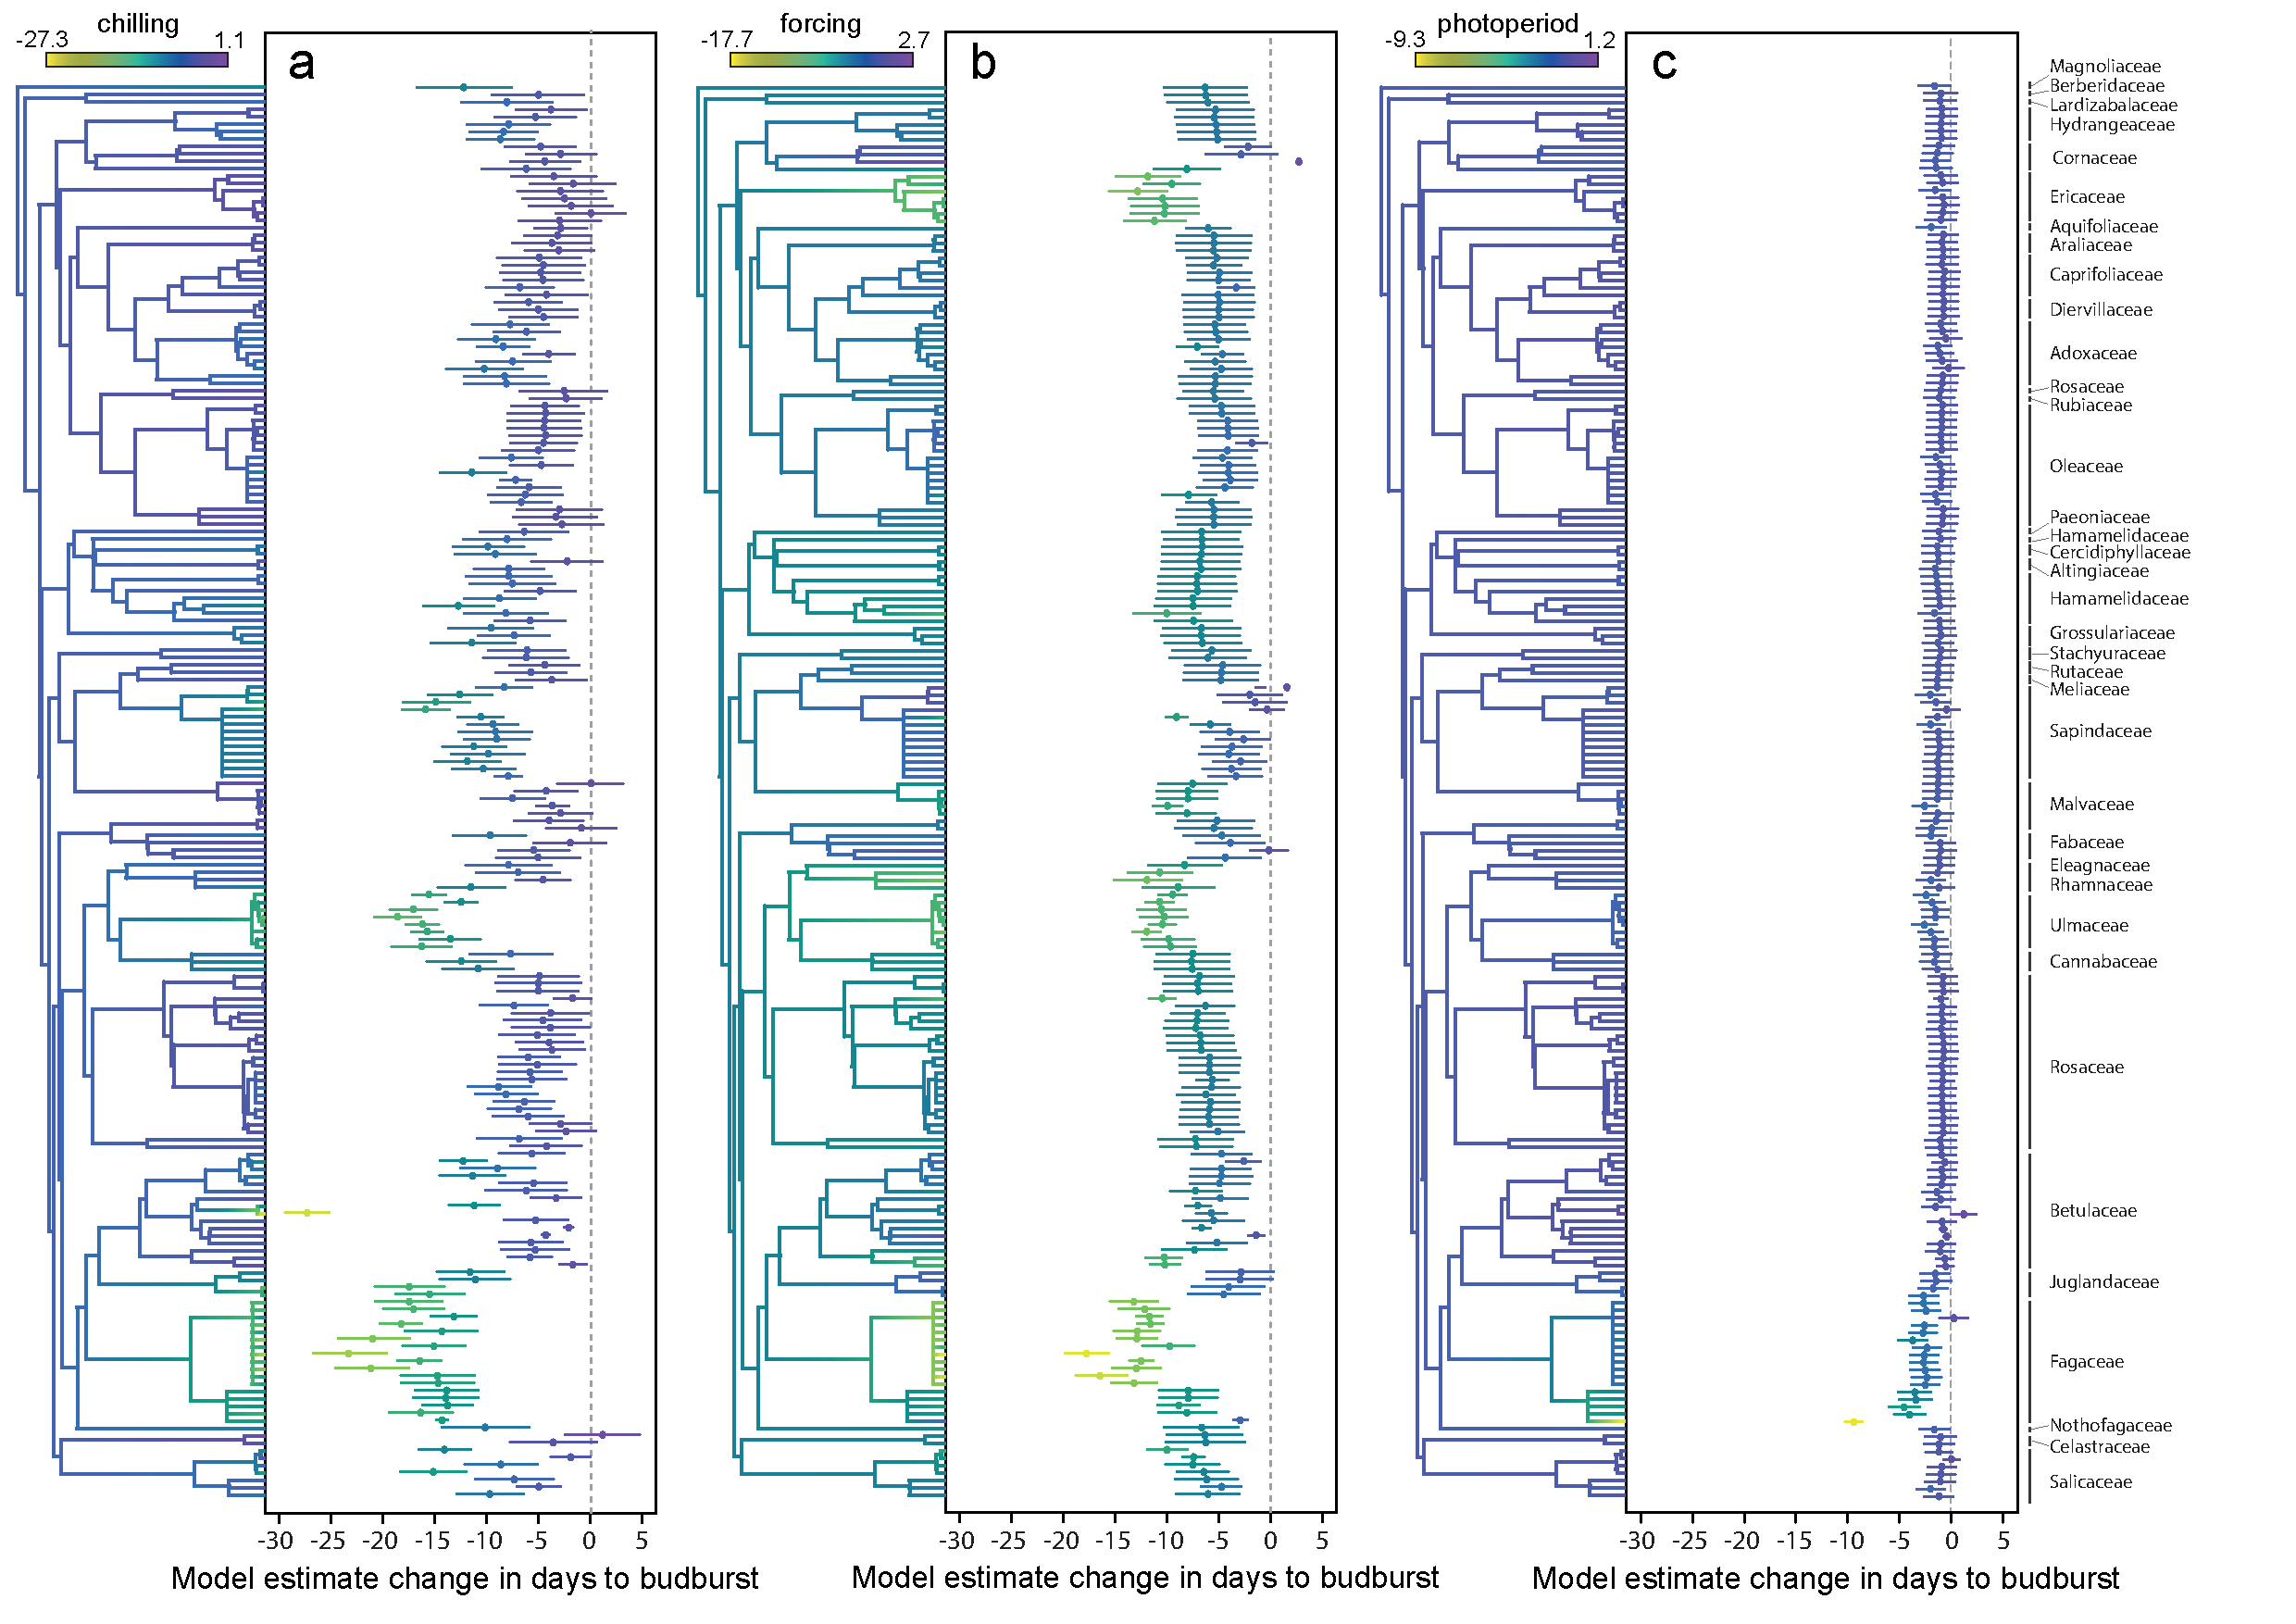
\includegraphics[width=16cm]{../../analyses/phylogeny/figures/Fig.1 phylo_muplots191_clades_nonames.pdf}
  \caption{\textbf{Phenological sensitivity to three environmental cues across 191 woody species estimated by a Phylogenetic Mixed Model.} The environmental cues are chilling (a), forcing (b) and photoperiod (c) measured as change in days to budburst per standardized unit ($z$-transformation) of the cues. The database used to fit the Phylogenetic Mixed Model comprised 44 studies, 191 species and 2940 observations. The same phylogenetic tree is shown in each panel, colored according to an estimation of ancestral character states, being the states at the tips the species sensitivities to a cue, as estimated by our hierarchical phylogenetic model. Species sensitivities are shown as mean values $+/-$ 50\% uncertainty intervals. Note that the color scale varies in each panel. Total tree depth is 81 My.}
  \label{fig:muplot_all}
  \end{center}
\end{figure}


\begin{figure} 
  \begin{center}
%  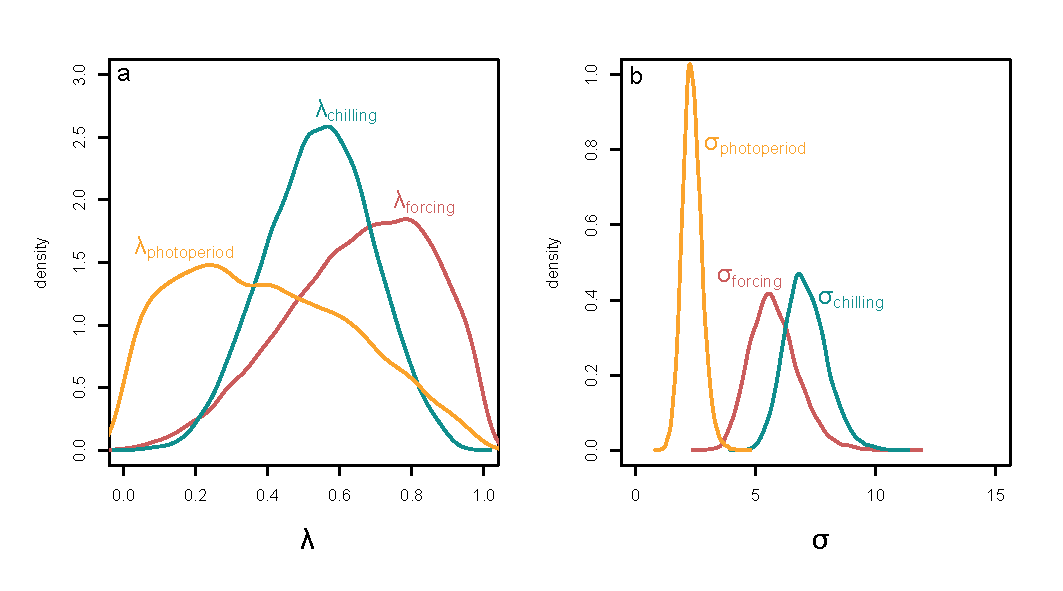
\includegraphics[width=14cm]{../../analyses/phylogeny/figures/Fig2_lambdas_sigmas.pdf}
  \caption{\textbf{Posterior distributions of phylogenetic parameters.} The lines show density plots comparing the lambda ($\lambda$) and sigma ($\sigma$) parameters estimated for each cue in the model: chilling (blue), forcing (red), and photoperiod (orange). Panels correspond to $\lambda$ (a) and $\sigma$ (b) from the phylogenetic model. The $\lambda$ parameter measures phylogenetic signal in each estimate of cue sensitivity (or how close species are similarly sensitive to a given cue, in a scale ranging from 0 to 1). The $\sigma$ parameter indicates evolutionary rate or accummulation of phenotypic variation with evolutionary time.}
  \label{fig:phylosig_all}
  \end{center}
\end{figure}

\begin{figure} 
  \begin{center}
%  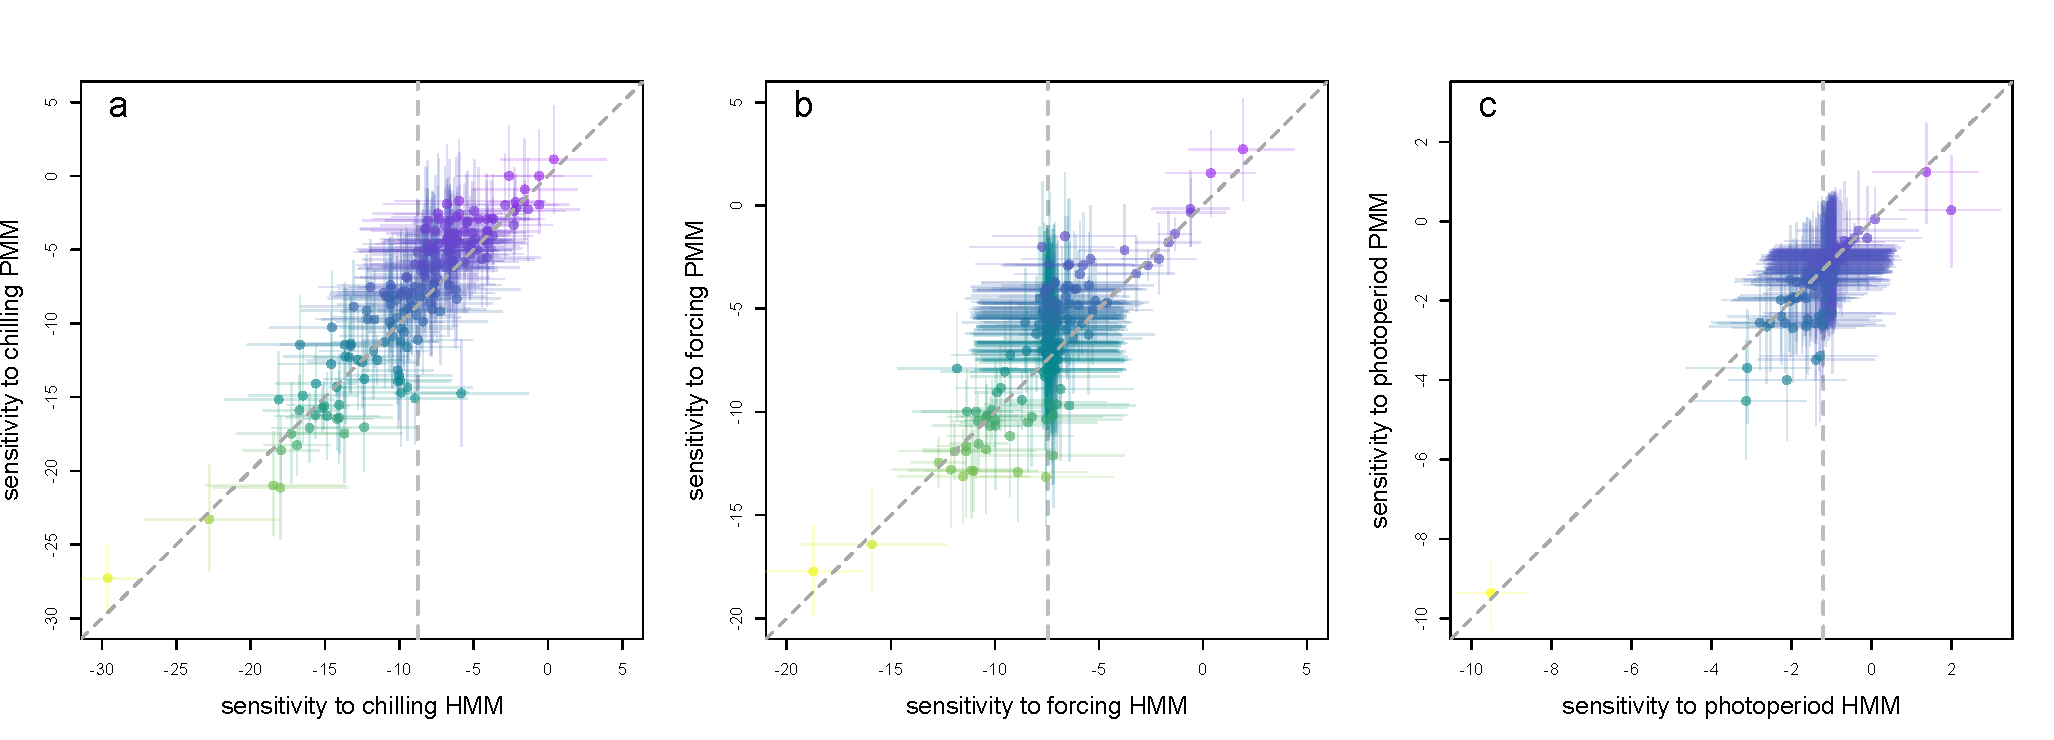
\includegraphics[width=14cm]{../../analyses/phylogeny/figures/Fig3_correlations_lambestvslamb0_cols.pdf}
  \caption{\textbf{Correlations between parameters estimated by the phylogentic and non-phylogenetic model.} The phylogenetic model(phylogenetic mixed model, PMM; $y$-axis) accounts for phylogenetic structure on each phenological cue, and the more commonly used hierarchical mixed model (HMM; $x$-axis) where species are exchangeable (where $\lambda$ is constrained to be equal to zero, $x$-axis). While species with large amounts of data may be estimated similarly by both models, in the more commonly used hierarchical model ($x$-axis) many species are pulled towards the overall average (shown by dashed grey vertical lines). The strength and prevalence of pulling across species is particularly obvious for forcing (b). Panels correspond to sensitivity to chilling (a), forcing (b), and photoperiod (c). Dashed grey 1:1 lines also shown. Species estimates are shown as mean values $+/-$ 50\% uncertainty intervals with estimate colors are in the same scale as in \ref{fig:phylosig_all}. Note that uncertainties of each species are higher in HMM than in PMM (Extended Data Fig. \ref{fig:pmmvshmm}). The database used to fit both models comprised 44 studies, 191 species and 2940 observations.}
  \label{fig:correls_angio}
  \end{center}
\end{figure}




\begin{figure} 
  \begin{center}
%  \includegraphics[width=16cm]{../../analyses/phylogeny/figures/Fig4_forecasting_diffstdpmm-lmm_pngnice.pdf}
  \caption{\textbf{Comparison of forecasts of phenological shifts resulting from a phylogenetic (PMM) and a non-phylogenetic but hierarchical (HMM) approach.} Phenological shifts were computed as the difference between predictions under current climate vs. a 2$^{\circ}$C warmer climate). Differences in forecasted shifts are negligible for well sampled species (\emph{Betula pendula}, $n = 311$, a), but can be substantially different for poorly sampled species in well-sampled clades (\emph{Acer campestre}, $n = 6$, b). The maps show the difference in number of days between the shifts predicted by PMM and HMM, with values colored according to histograms in panel c (days here are relative to start of forcing conditions, not calendar days). See Supplementary Information for details on forecast calculation.}
  \label{fig:forecast}
  \end{center}
\end{figure}



\clearpage


\section*{References} 
\bibliography{phylorefs}
\bibliographystyle{naturemag}


\section*{Data availability}
Our data comprises phenological responses of 191 species to experimental treatments of temperature and daylight. Data were subset from a larger existing dataset published by the authors (OSPREE, doi:10.5063/F1CZ35KB), which assembles the largest available dataset on experimentally determined woody plant phenology. The data included all budburst experiments where we could quantify chilling, forcing and photoperiod levels for target species, resulting in 44 studies from 33 papers. All data supporting the findings of this study are publicly available in GitHub \url{https://zenodo.org/records/10902899}.

\section*{Code availability}
Data analyses were performed in R and Bayesian Hierarchical and Phylogenetic Mixed Models (HMM and PMM, respectively) were performed within the Stan environment. All Stan and R custom code to run models and visualize results is publicly available in GitHub \url{https://zenodo.org/records/10902899}.




\end{document}
